% BEGIN PREAMBEL
\documentclass[9pt]{beamer}
\usepackage[british]{babel}
\usepackage[latin1]{inputenc}
\usepackage{multimedia}
\usepackage{amsmath,amsfonts,amssymb}
\usepackage{upgreek}
\usepackage{pgfpages}
\usepackage[version=3]{mhchem}
\usepackage{lmodern}
\usepackage{graphicx}
\usepackage{multicol}
\usepackage{xcolor}
\usepackage{wrapfig}
\usepackage{siunitx}
\newcommand{\as}{\\[14pt]}
\newcommand{\s}{\\[7pt]}
\newcommand{\is}{\\[2pt]}
\newcommand{\no}{\noindent}
\newcommand{\ka}{\hspace*{0.5cm}}
\newcommand{\ma}{\hspace*{1cm}}
\newcommand{\ga}{\hspace*{1.5cm}}
\newcommand{\li}{\left|}
\newcommand{\re}{\right|}
\newcommand{\const}{\text{const.}}
\newcommand{\z}{\text}
\newcommand{\terminal}[1]{\colorbox{black}{\textcolor{white}{{\fontfamily{phv}\selectfont \scriptsize{#1}}}}}
\newcommand{\plugin}[1]{\textit{\flq#1\frq}}
\usetheme{Boadilla}
\graphicspath{ {Pics/} }
\usecolortheme{beaver}
\useoutertheme{miniframes}
\beamertemplatenavigationsymbolsempty
\makeindex
\title[Layer1 Module]{Updates on Layer1 Module}
\author[M. Reichmann]{Michael Reichmann}
\institute[\textbf{\textit{ETH}}\scalebox{.6}{\textit{Z\"{u}rich}}]{Swiss Federal Institute of Technology Zurich}
\AtBeginSection{\frame{\sectionpage}}
% END PREAMBEL
\begin{document}
% ============================
% BEGIN TITLE PAGE
% ============================
\begin{frame}
	\begin{center}
		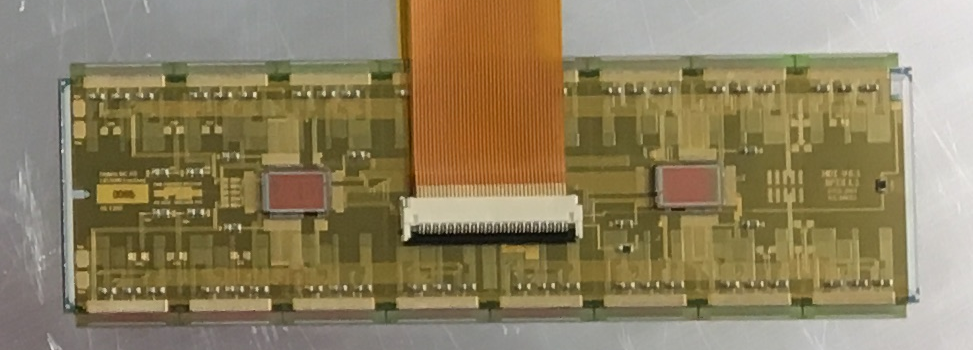
\includegraphics[width=8cm]{Mod}
	\end{center}
	\begin{alertblock}{
		\begin{center}
			\textbf{Updates on Layer1 Module \today}
		\end{center}}
		\vspace*{10pt}
		\begin{center}\small
		Michael Reichmann
		\end{center}\normalsize
	\end{alertblock}
\end{frame}
% END
% ============================
% BEGIN TABLE OF CONTENTS
% ============================
\begin{frame}[allowframebreaks]
	\frametitle{Table of contents}
	\tableofcontents   % [pausesections]
\end{frame}
% END
% ====================================================================================
% STOCK
% ====================================================================================
\section{Stock}
% ============================
\begin{frame}
	\begin{itemize}
		\item two Layer1 Modules at PSI
		\begin{itemize}
			\item one with TBM09 (Token Bit Manager)
			\item one with the new TBM10 $\rightarrow$ electrical shortcut
		\end{itemize}
		\item both TMBs meant to be used as pair (afaik)
	\end{itemize}
	\begin{center}
		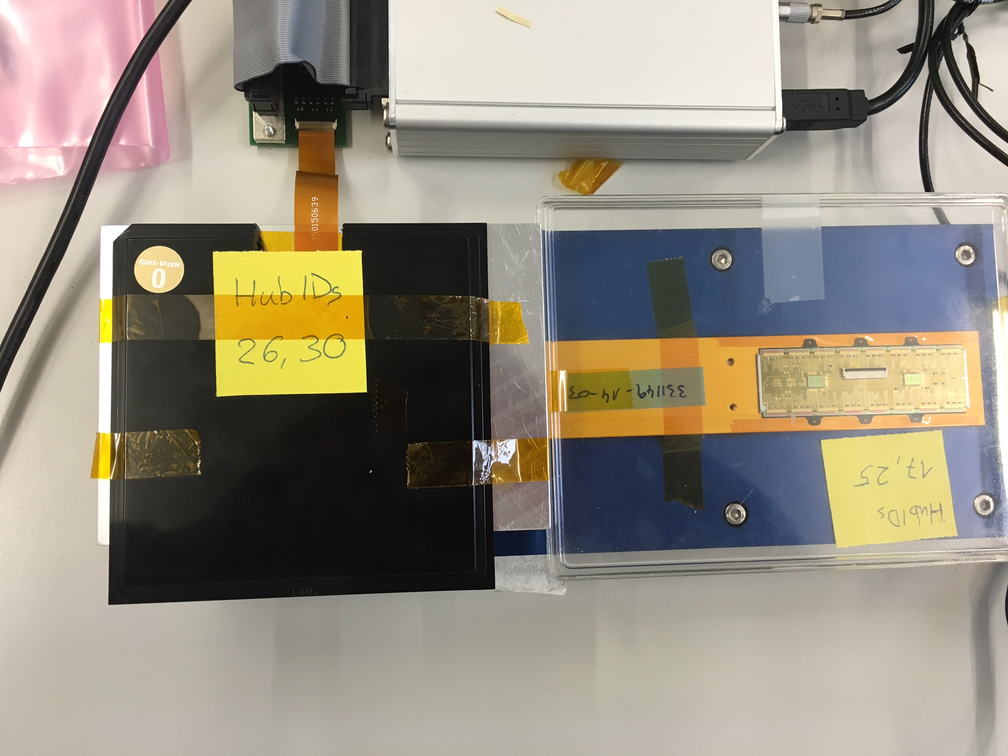
\includegraphics[width=8cm]{bothMod}
	\end{center}
\end{frame}
% ====================================================================================
% CONFIG
% ====================================================================================
\section{Configuration Files}
% ============================
\begin{frame}
	\underline{\textbf{configParameters.dat}}
	\begin{itemize}
		\setlength{\itemsep}{\fill}
		\item hubID: wire bonded address of the TBM
		\item changing hubID from value to vector$<$value$>$
		\item adding function to read in multiple hubIDs
		\item default setting is {31} (vector with one entry) ( 31 = default address of the old modules)
		\item adding function to turn a vector into a string
		\item fixing writeConfigParameterFile(): multiple hubIDs correctly written back to file
	\end{itemize}
	\vspace*{.7cm}
	\underline{\textbf{tbmParameters*.dat}}
	\begin{itemize}
		\setlength{\itemsep}{\fill}
		\item TBM timing config files were incorrectly saved
		\item fixing the save files names 
	\end{itemize}
\end{frame}
% ====================================================================================
% 4th APRIL
% ====================================================================================
\section{4th April}
% ============================
\begin{frame}
	\begin{itemize}
		\setlength{\itemsep}{\fill}
		\item some code style improvements
		\item Wolfram improving speed of timing test by assigning less buffer size
		\item module heating problem
		\item checking timings
		\item weird pixel maps and tornado plots $\rightarrow$ add plots
		\item no history of the modules and sensors...
	\end{itemize}
\end{frame}
% ============================
\subsection{Heating-Up of the Modules}
\begin{frame}
	\begin{itemize}
		\setlength{\itemsep}{\fill}
		\item TBM10 module was still in black transportation box
		\item module heats up significantly while pXar is running 
			\begin{itemize}
				\item box was hot by touch
			\end{itemize}
		\item DACs and timing T-dependent
		\item moving module from the box onto a aluminum block as heat spreader
		\item module slightly bent while removing from the box
		\item Tilman and Wolfram could not find any history of the modules
		\item module still working, bump bonds map did not look too bad $\rightarrow$ add pic
		
	\end{itemize}
	\begin{center}
		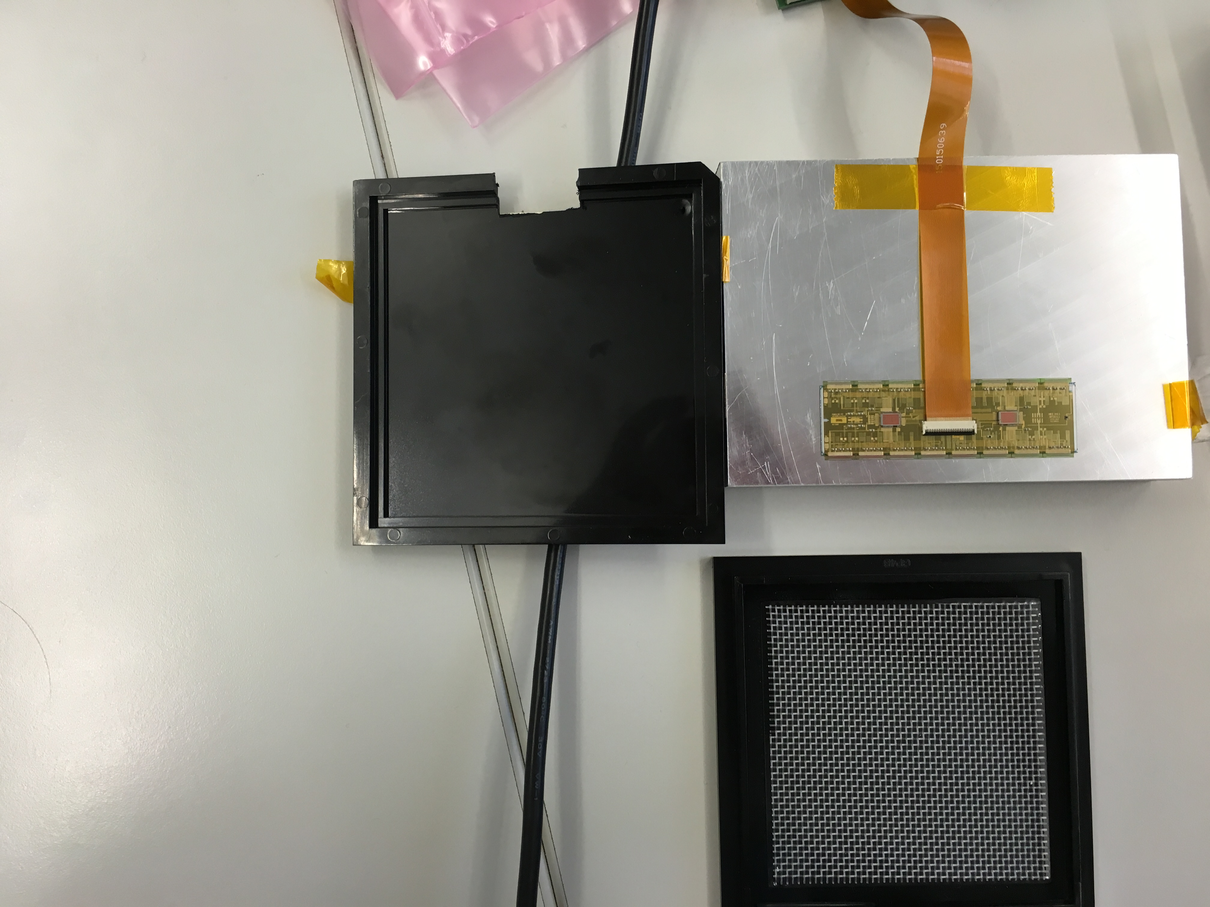
\includegraphics[width=6cm]{Module}
	\end{center}
\end{frame}
% ============================
\subsection{Pretest / Timing}
\begin{frame}
	\begin{itemize}
		\setlength{\itemsep}{\fill}
		\item pretest not fully working
		\begin{itemize}
			\item some pixel maps missing circular shapes
			\item tornado plots twisted and cut apart
			\item no timing test used for TBM09 and TMB10
		\end{itemize}
		\item need to debug Wolframs timing test for the new module
		\item started to dig into the code
	\end{itemize}
\end{frame}
% DOCUMENT END
\end{document}

